\documentclass[border=3mm,tikz]{standalone}
\usepackage{pgfplots}

\pgfplotsset{compat=1.10}
\usepgfplotslibrary{fillbetween}
\usetikzlibrary{patterns}

\begin{document}

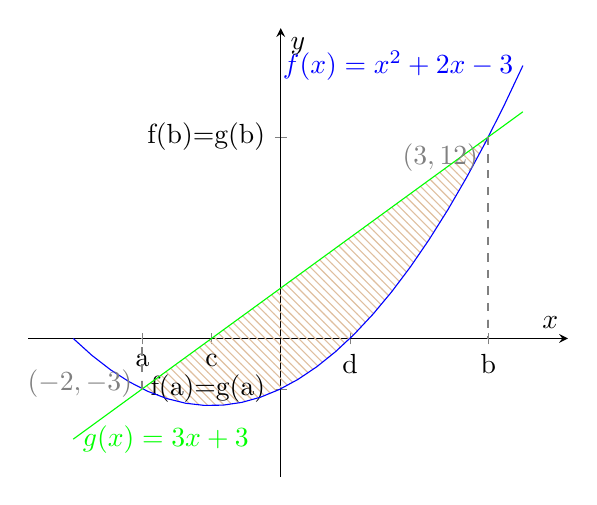
\begin{tikzpicture}
\begin{axis}[axis lines=middle,
            xlabel=$x$,
            ylabel=$y$,
            enlargelimits,
            ytick={-3,12},
            yticklabels={f(a)=g(a),f(b)=g(b)},
            xtick={-2,-1,1,3},
            xticklabels={a,c,d,b}]
\addplot[name path=F,blue,domain={-3:3.5}] {x^2+2*x-3} node[pos=1, left]{$f(x)=x^2+2x-3$};

\addplot[name path=G,green,domain={-3:3.5}] {3*x+3}node[pos=0, right]{$g(x)=3x+3$};

\addplot[thick, samples=50, smooth,gray, name path=three, dashed] coordinates {(-2,-3)(-2,0)} node[pos=.1, left]{$(-2,-3)$};
\addplot[thick, samples=50, smooth,gray, name path=three, dashed] coordinates {(3,12)(3,0)} node[pos=.1, left]{$(3,12)$};

\addplot[pattern=north west lines, pattern color=brown!50]fill between[of=F and G, soft clip={domain=-2:3}];

%\node[coordinate,pin=30:{$A$}] at (axis cs:3.8,3){};

\end{axis}
\end{tikzpicture}


\end{document}
